\chapter{The World Bank's Data}\label{chap_data}

As shown on chapter \ref{chap_intro}, collecting the necessary data for any Data Science project is almost always a huge task because the reality tends to be that some of the most relevant variables commonly go unmeasured or are private. This project uses  two types of data, private and public. This chapter describes the two main types of data used for this project.
Section \ref{sec_inv_data} describes the characteristics of private data and the scope it has. It also explains about the confidentiality agreement Integrity Vice Presidency (INT) offered this project in exchange for investigations data. Section \ref{sec_public_data} explains how to download public data from the Wold Bank's servers using coding tools.

\section{Private data}
\subsection{Investigations} \label{sec_inv_data}

The most valuable data for this project was the private data which the partners at INT made available for the project while maintaining a spirit of openness. A confidentiality agreement was signed in order to give access to the investigations database. The only condition was that all the data and analyses had to be stored and processed on a remote server with an encryption and security measurements that satisfied the World Bank's standards. 

In this case the server was an Amazon Web Service's (AWS), Amazon Elastic Compute Cloud (Amazon EC2) machine. EC2 is a web service that provides resizable compute capacity in the cloud. It is designed to make web scale cloud computing easier for developers\footnote{``Amazon EC2’s simple web service interface allows you to obtain and configure capacity with minimal friction. It provides you with complete control of your computing resources and lets you run on Amazon’s proven computing environment. Amazon EC2 reduces the time required to obtain and boot new server instances to minutes, allowing you to quickly scale capacity, both up and down, as your computing requirements change. Amazon EC2 changes the economics of computing by allowing you to pay only for capacity that you actually use. Amazon EC2 provides developers the tools to build failure resilient applications and isolate themselves from common failure scenarios.'' \parencite{aws_es2}}. For more details on how to setup an AWS computer see \parencite{aws_start} and appendix \ref{chap_software}. In other words, the data was stored in an AWS machine on the cloud that had an encrypted folder with the specific files. Since all the data had to stay on the cloud, all the processing had to be done on the cloud too. For this purpose, a server running \texttt{Python} and \texttt{R} was hosted at an AWS computer. 


\subsubsection{Description}

The investigations data consists of nearly 13,000 cases, of which over half are Fraud and Corruption. 377 are labeled as Collusion. These are from the ``Allegation Category'' column, Notably, allegation categories include Fraud, Corruption, and Fraud \& Corruption. It is possible for a case's description to just say Fraud and for its allegation category to still be Fraud and Corruption. For the purpose of this project, each of these 3 categories were considered as the same (i.e. all ``Fraud and Corruption''). Allegations also include a ``Allegation Sub-Category''. Collusion is sometimes listed as a sub-category, for example: Allegation Category: Fraud and Corruption or Allegation Sub-Category: Bid Manipulation/Collusion. The Unit of analysis is the investigations data is the ``Subject'' which refers to the entity that was investigated. Mostly this variable refers to companies and people, but on occasion other entities on a project may be subjects of investigation, for example the coordinating agency. For example Case \# A-AAA-1234-5678, the subject is: Country's X Ministry of Education. In procurement data it shows up in ``Implementing Agency'' differently.
    
The Labels in the investigations are very different and specific to each investigation case. The most relevant label will be the Allegation Outcome's column. The most frequent outcomes for a case are ``Substantiated'', which means that the Subject was found to be guilty of the Allegation, ``Unfounded'', which means that the Subject was found to be  innocent of the allegation, and ``Unsubstantiated'', which means that the investigation did not have the necessary means to conclude that the subject was  guilty, but neither does it have to conclude that the subject is innocent. Substantiated and Unsubstantiated occur in roughly equal quantities, while Unfounded is fairly rare. There are other labels like ``We kicked it to another organization''.

The identities of the cases within the investigations data include that about 80\% of the data has either the name of the accused (the majority) or the project number (about a third). These are in the Subject and Project Number columns, respectively. That means about 20\% of the data appears to be ``lost'', in that we can't match it up to any procurement data. There is potentially other information in the ``Title'' field, but it is unstructured. There could theoretically be information in other fields, but they are not as rich.

There are among 1000 different sectors but most of them are mixed sectors and have not been previously cleaned. For example, when an investigation involves cases that cover sectors such as transportation and urban development there can be the case that you find a Transportation sector, a Urban Development sector and a Transportation \& Urban Development Sector. For the specifics of the model, this project works with sector specific as they are, this meaning that, for the project, the three cases mentioned before are considered to be different sectors. By doing so, there are about 205 sectors.


\section{Public data}\label{sec_public_data}



Fortunately for the project, not all the data was private. This work uses the Open Data\footnote{Go to \cite{wb_data}.}  and the Data Bank websites from the World Bank, which offer free access to comprehensive, downloadable indicators about development in countries around the globe. 

Public data from the World bank comes from different databases. They are generated at different sections within the World Bank so each indicator can be obtained form a specific database according to its nature. For example, all the Development indicators can be obtained at the World Bank's World Development Indicators database, indicators regarding how easy it ts to do business in each specific country could be obtained from the Doing Business database and indications regarding world's populations can be obtained at the Health Nutrition and Population Statistics database.\footnote{Different databases include:
Africa Development Indicators, Statistical Capacity Indicators, Country Policy and Institutional Assessment (CPIA), Country Partnership Strategy for India, Corporate Scorecard, Doing Business, Exporter Dynamics Database: Country-Year, Education Statistics, Enterprise Surveys, Global Findex ( Global Financial Inclusion database), G20 Basic Set of Financial Inclusion Indicators, Gender Statistics, Global Economic Monitor, GEP Economic Prospects, Global Financial Development, Global Economic Monitor (GEM) Commodities, Global Partnership for Education, Global Social Protection, Health Nutrition and Population Statistics, Health Nutrition and Population Statistics by Wealth Quintile, Health Nutrition and Population Statistics: Population estimates and projections, International Development Association - Results Measurement System, INDO-DAPOER, International Debt Statistics, Jobs for Knowledge Platform, LAC Equity Lab, Millennium Development Goals, Povstats, Quarterly Public Sector Debt, Quarterly External Debt Statistics/GDDS (New), Quarterly External Debt Statistics/SDDS (New), Readiness for Investment in Sustainable Energy (RISE), Sustainable Energy for All, Subnational Malnutrition Database, Subnational Poverty, Subnational Population, Wealth accounting, World Development Indicators and the  Worldwide Governance Indicators.}

A good practice in Data Science is to generate code so that all results can be easily replicated. That was the reason why, for this project all the data that the World Bank bank provides publicly by an Application Programming Interface (API) was collected with reliable code. Thanks to prior World Bank's work, accessing the World Bank Data APIs with code in languages such as \texttt{Python}, \texttt{R}, \texttt{Ruby} and \texttt{Stata} is a simple task. The World Bank has a blog where they explain in detail how to use the APIs. See the \cite{wb_api}, the \cite{wb_python} and the \cite{wb_r} for more details on how to do this. To put things in context, \texttt{Python} and \texttt{Ruby} are general-purpose programming languages, and \texttt{Stata} and \texttt{R} are programming environments optimized for statistics. They're all widely used in the business and academic worlds. The World Bank generates modules to those languages which help users to connect to the World Bank Development Indicators API and access the latest data.

For example, in \texttt{python}, the \texttt{wbdata} module by Oliver Sherouse offers easy access to all the data in the World Bank's APIs. It also plays nicely with Wes McKinney’s  \texttt{pandas} analysis library\footnote{See appendix \ref{chap_software} for \texttt{pandas} details.}. \texttt{Wbdata} is a simple python interface to find and request information from the World Bank's various databases, either as a dictionary containing full meta data or as a \texttt{pandas} Data Frame. Currently, \texttt{wbdata} wraps most of the World Bank API, and also adds some convenience functions for searching and retrieving information.

In \texttt{R}, the \texttt{WDI} module by Vincent Arel-Bundock offers convenient access to the data in the World Bank's API. For fast searching, the \texttt{WDI} package ships with a local list of available data series. This local list can be updated to the latest version using the \texttt{WDIcache} function \parencite{wb_r}. Similar tools are available to languages such as Ruby and Stata.

Given that, the public data used in this project can be divided in two sets; first, the World Bank's World Development Indicators, which can be obtained by using the API and the packages mentioned; and, second, all the historical and major awards given by the World Bank to all developing countries from 1990 to 2014. 


\subsection{World Development Indicators}

The World Bank has a major data base called: World Development Indicators (WDI). WDI is the primary World Bank collection of development indicators, compiled from officially recognized international sources. This database represents the most current and accurate global development data available, and includes national, regional and global estimates. For the purpose of this work, the indicators selected such that prediction of corruption, collusion and fraud would not be attainable to specific country variables such as country or country region. This is was because the World Bank can not start investigation cases in specific countries just because different countries tend to have different levels of corruption. Unfortunately, those types of variables can have, in some times, much better prediction rates but the policies at the World Bank prevents a model of having them for discretion and discrimination arguments.

Also, the World Bank has around 16,000 different indicators the project could use, but being this big, and according to purpose of this project, only a few indicators were selected. The next list shows the ones that were considered. This list includes indicators related to the private sector and trade among countries which is the theme the project is targeting.

\begin{description}
\item[IC.BUS.DISC.XQ]	Private Sector \& Trade: Business environment. Business extent of disclosure index (0=less disclosure to 10=more disclosure)	Disclosure index measures the extent to which investors are protected through disclosure of ownership and financial information. The index ranges from 0 to 10, with higher values indicating more disclosure.
\item[IC.FRM.CMPU.ZS]	Private Sector \& Trade: Business environment. Firms competing against unregistered firms (\% of firms).
\item[IC.FRM.CORR.ZS]	Private Sector \& Trade: Business environment	Informal payments to public officials (\% of firms).
\item[IC.FRM.INFM.ZS]	Private Sector \& Trade: Business environment	Firms that do not report all sales for tax purposes (\% of firms).
\item[IC.LGL.CRED.XQ]	Private Sector \& Trade: Business environment	Strength of legal rights index (0=weak to 10=strong).
\item[IC.LGL.DURS]	Private Sector \& Trade: Business environment	Time required to enforce a contract (days).
\item[IC.TAX.GIFT.ZS]	Private Sector \& Trade: Business environment	Firms expected to give gifts in meetings with tax officials (\% of firms).
\item[IQ.CPA.PROP.XQ]	Public Sector: Policy \& institutions	CPIA property rights and rule-based governance rating (1=low to 6=high).
\item[IQ.CPA.TRAN.XQ]	Public Sector: Policy \& institutions	CPIA transparency, accountability, and corruption in the public sector rating (1=low to 6=high).
\item[NY.GDP.PCAP.CD]	Economic Policy \& Debt: National accounts: USD at current prices: Aggregate indicators	GDP per capita (current US\$).
\item[SE.PRM.PRSL.ZS]	Education: Efficiency	Persistence to last grade of primary, total (\% of cohort).
\item[SI.POV.GINI]	Poverty: Income distribution GINI index.
\item[SL.UEM.TOTL.NE.ZS]	Social Protection \& Labor: Unemployment	Unemployment, total (\% of total labor force) (national estimate).
\end{description}

The code to download WDI can be seen at the Appendix \ref{chap_code} in code \ref{code_wdi}. This code can easily replicate results. For the purpose of this work, the code in \ref{code_wdi} downloads data for the countries within the countries from the investigations data, those countries define the countries list for this work.

As it can be seen from the figures \ref{fig_wdi_bribes} to \ref{fig_wdi_time_contract}, There are many differences among regions in the world. 
For example, on figure \ref{fig_wdi_bribes} that countries such as Vietnam in East Asia \& Pacific, Grece, Portugal in Europe \& Central Asia, Iraq in the Middle East \& North Africa, Pakistan in South Asia and Democratic Republic of Congo, show high levels of percentage of Bribes to tax officials with levels higher than 40\%. On the other hand, countries such as Micronecia in East Asia \& Pacific, Slovenia, Sweden and Stonia in Europe \& Central Asia, Chile, Mexico, Colombia and Uruguay in Latin America \& Caribian, Israel and Tunisia in the Middle East \& North Africa, Nepal and Sri Lanka in South Asia and South Africa and Rwuanda in Sub-Saharan Africa show low levels of percentage of Bribes to tax officials with numbers lower than 10\%.
Figure \ref{fig_wdi_firms} shows the percentage of firms competing against informal firms. This indicator shows significant differences in each region. In the East Asia, Toga has the highest percentage near to 80\% against Philippines and Lao PDR with just about 25\%. In Europe and Central Asia, Kosovo has around 70\% against Slovenia and Uzbekistan with 25\%. In Latin America and the Caribbean, Bolivia, Uruguay and Mexico reach as far as 75\% against Panama with levels near to 25\%. In the Middle East and North Africa, Argelia has about 70\% and Jordan and Israel just about 20\%. In South Asia, Nepal and India have the highest levels with 50\%, where Bhutan and Pakistan have around 25\%. The highest levels are in Sub Saharan Africa where countries such as Sudan, Chad, Cameroon and Niger reach up to 80\% against Erittrea with levels higher than 25\%.
Now, figure \ref{fig_wdi_pays} shows the percentage of Payments to public officials where clearly, one more time, countries in Sub Saharan Africa have the highest levels like Guinea, Democratic republic of Congo, Republic of Congo and Cameroon reach up to 80\%.Countries like Syrian Arab Republic and Argelia in the Middle East, Kyrgyz Republic and Ukraine in Europe and Central Asia, Cambodia and Vietnam in East Asia, Paraguay in Latin America and Bangladesh in South Asia present also high levels near to 65\% in contrast with countries such as Sudan and Cabo Verde in Sub Saharan Africa, Israel and Tunisia in the Middle East and North Africa, Spain, Ireland and Montegro in Europe and Central Asia, Fiji, China and Tonga in East Asia and the Pacific, Mexico, Uruguay and Colombia in Latin America and Caribbean, India and Nepal in South Asia, present very low levels near to 20\%.
Finally, figure \ref{fig_wdi_time_contract} shows the mean time to enforce contracts in each country in hours. Differences are very radical. 
 In  East Asia, Timor-Leste has the highest number near to 1500 hours (63 days) against Singapore and New Zeland with just about 200 hours (9 days). In Europe and Central Asia, Slovenia and Italy it takes about 1300 (55 days) against Russian Federation, Finland and Luxemburg where it takes about 180 (8 days). In Latin America and the Caribbean, Suriname, Guatemala and Colombia have the longer time with about 1400 hours (58 days) against Mexico and Antigua \& Barbuda near to 350 (14 day). In the Middle East and North Africa,  in Djibouti and Egypt Arab Republic it takes near to 1200 hours (50 days) where in Malta, Moroco and Iraq just takes about 500 hours (20 days). As a reference, in USA and Canada it takes about 500 hours (20 days). In South Asia in countries such as Afghanistan and Banghladesh it takes about 1500 hours (63 days) and in Bhutan just about 250 (10 days). In the Sub Saharan Africa, the record of highest time goes to Guinea - Bissau with times up to 1700 hours (70 days) and the lower to South Sudan with just about 250 hours (10 days).

 Appendix \ref{chap_countries} show the figures of all the other indicators used in this project obtained with the package WDI\parencite{wb_r} and the code from appendix \ref{chap_code}.

 These indicators were chosen because each one of them suggest that variances within them show an impact on how many contracts present substantiated cases of corruption, collusion, coercion and fraud among the contracts that the World Bank have given to development projects in those countries. As chapter \ref{chap_procurements} says and figures \ref{fig_cum_value} to \ref{fig_proposals}  suggest, differences in the indicators among countries and regions might be clues to identify malicious contracts. 

\begin{figure}[H]
\begin{center}
\caption{WDI: \% of Bribes to tax officials per Country/Region}
\label{fig_wdi_bribes}
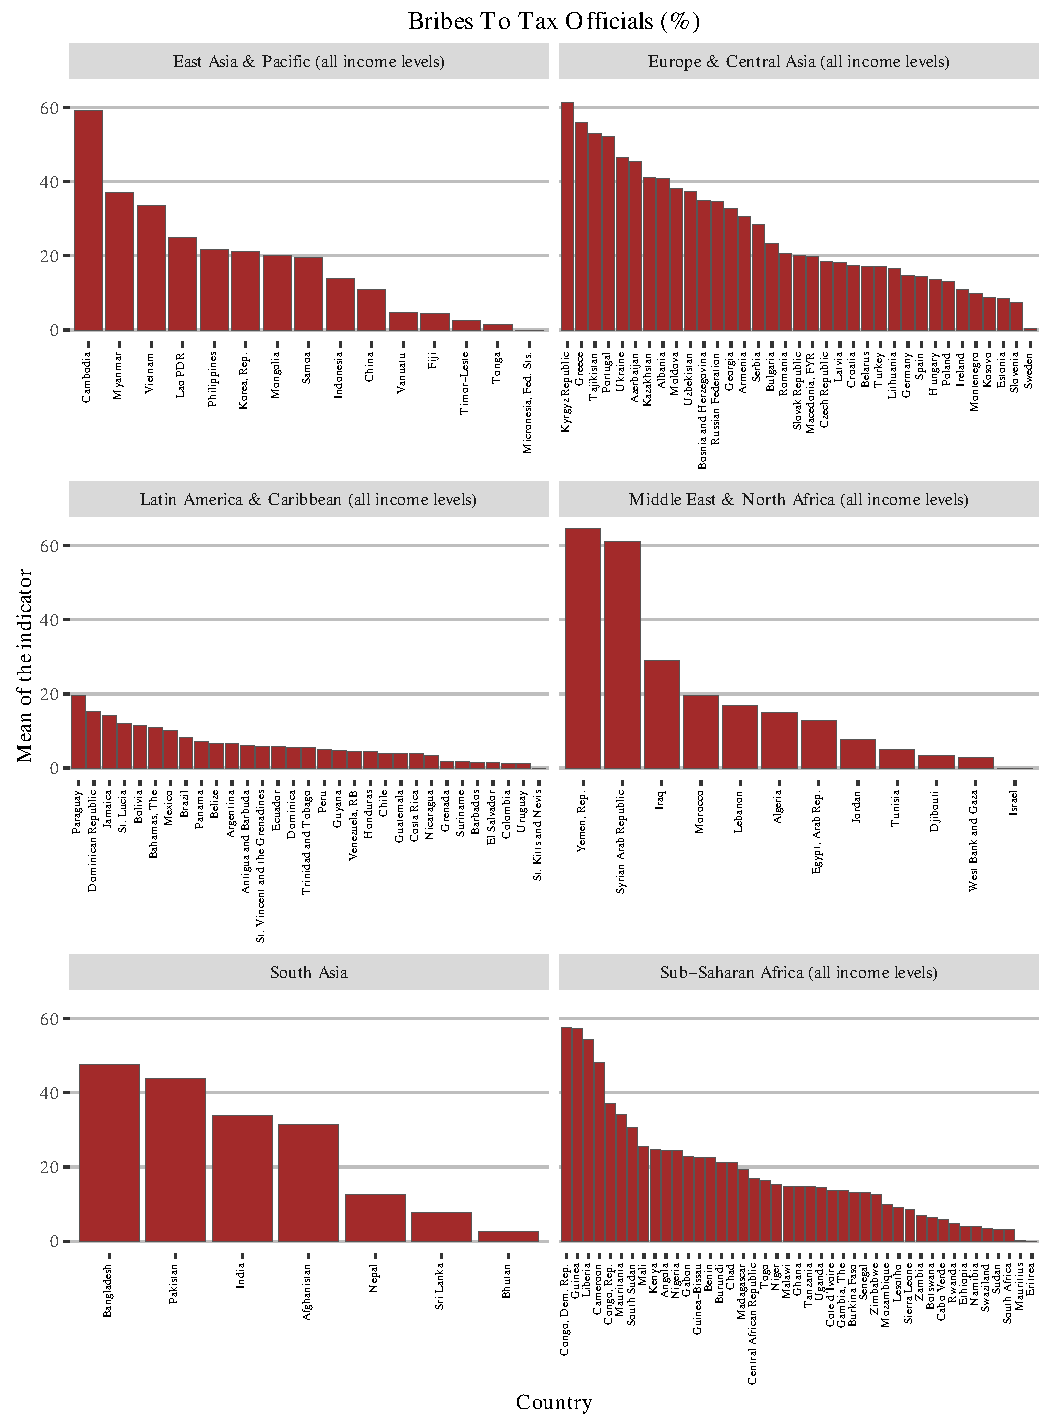
\includegraphics[max height=.9\textheight]{../img/wdi_bribes_to_tax_officials_perc.pdf}
\end{center}
\noindent \footnotesize{\textbf{Source:} Own creation and data obtained with package \texttt{WDI}, see the \cite{wb_r}.}
\end{figure}

\begin{figure}[H]
\begin{center}
\caption{WDI: \% of Firms competing against informal firms per country/Region}
\label{fig_wdi_firms}
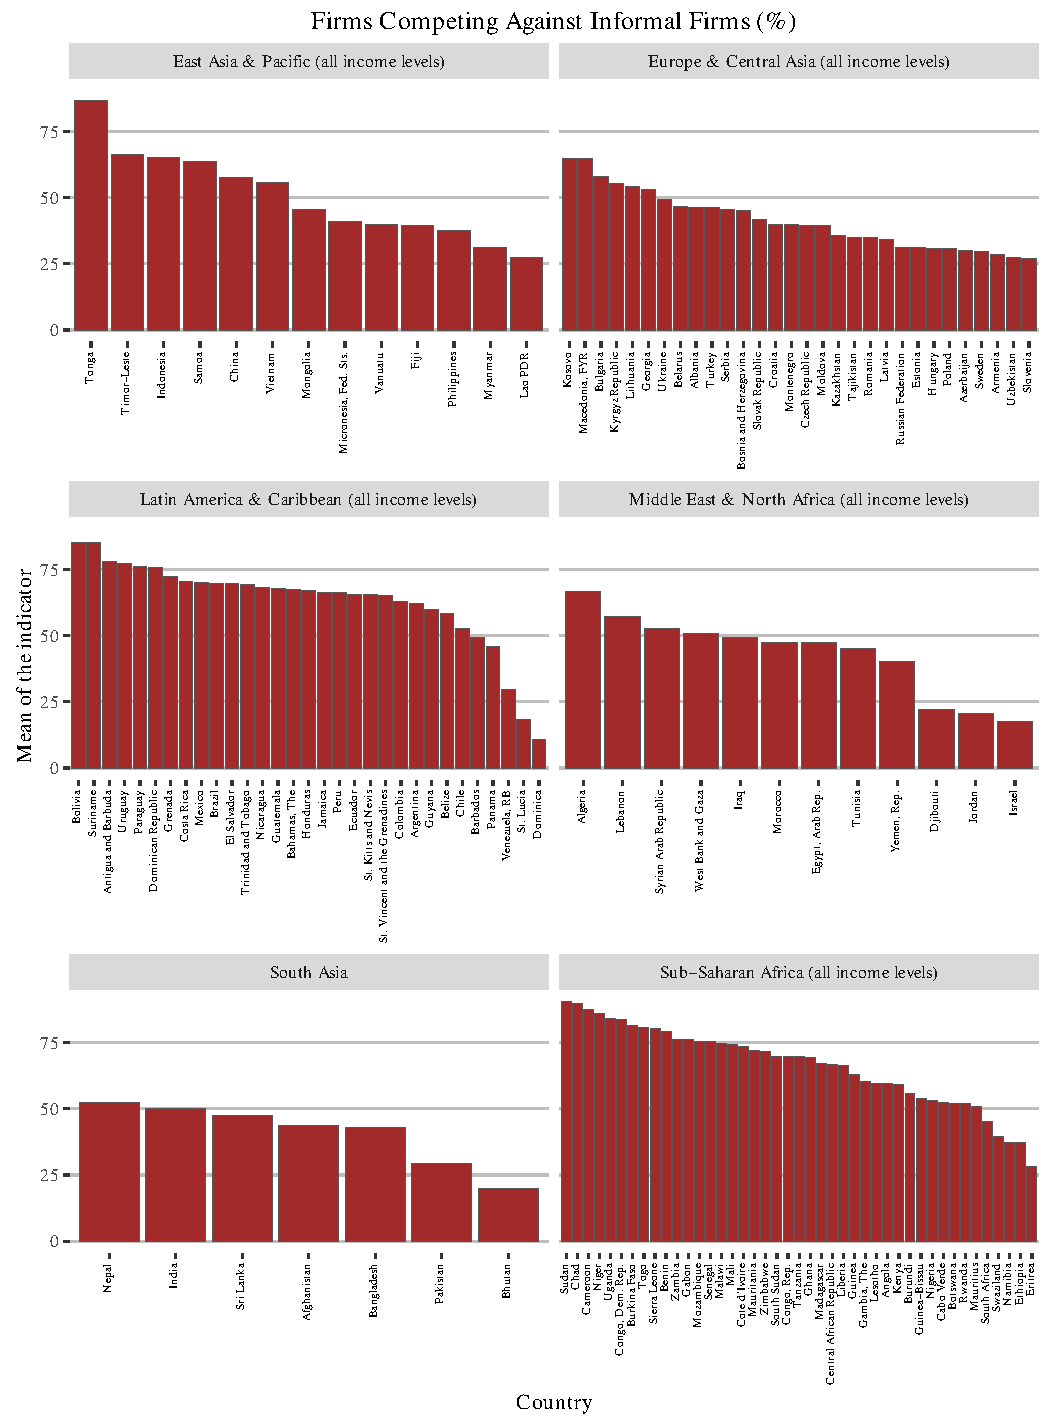
\includegraphics[max height=.9\textheight]{../img/wdi_firms_competing_against_informal_firms_perc.pdf}
\end{center}
\noindent \footnotesize{\textbf{Source:} Own creation and data obtained with package \texttt{WDI}, see the \cite{wb_r}.}
\end{figure}

\begin{figure}[H]
\begin{center}
\caption{WDI: \% of Payments to public officials per Country/Region}
\label{fig_wdi_pays}
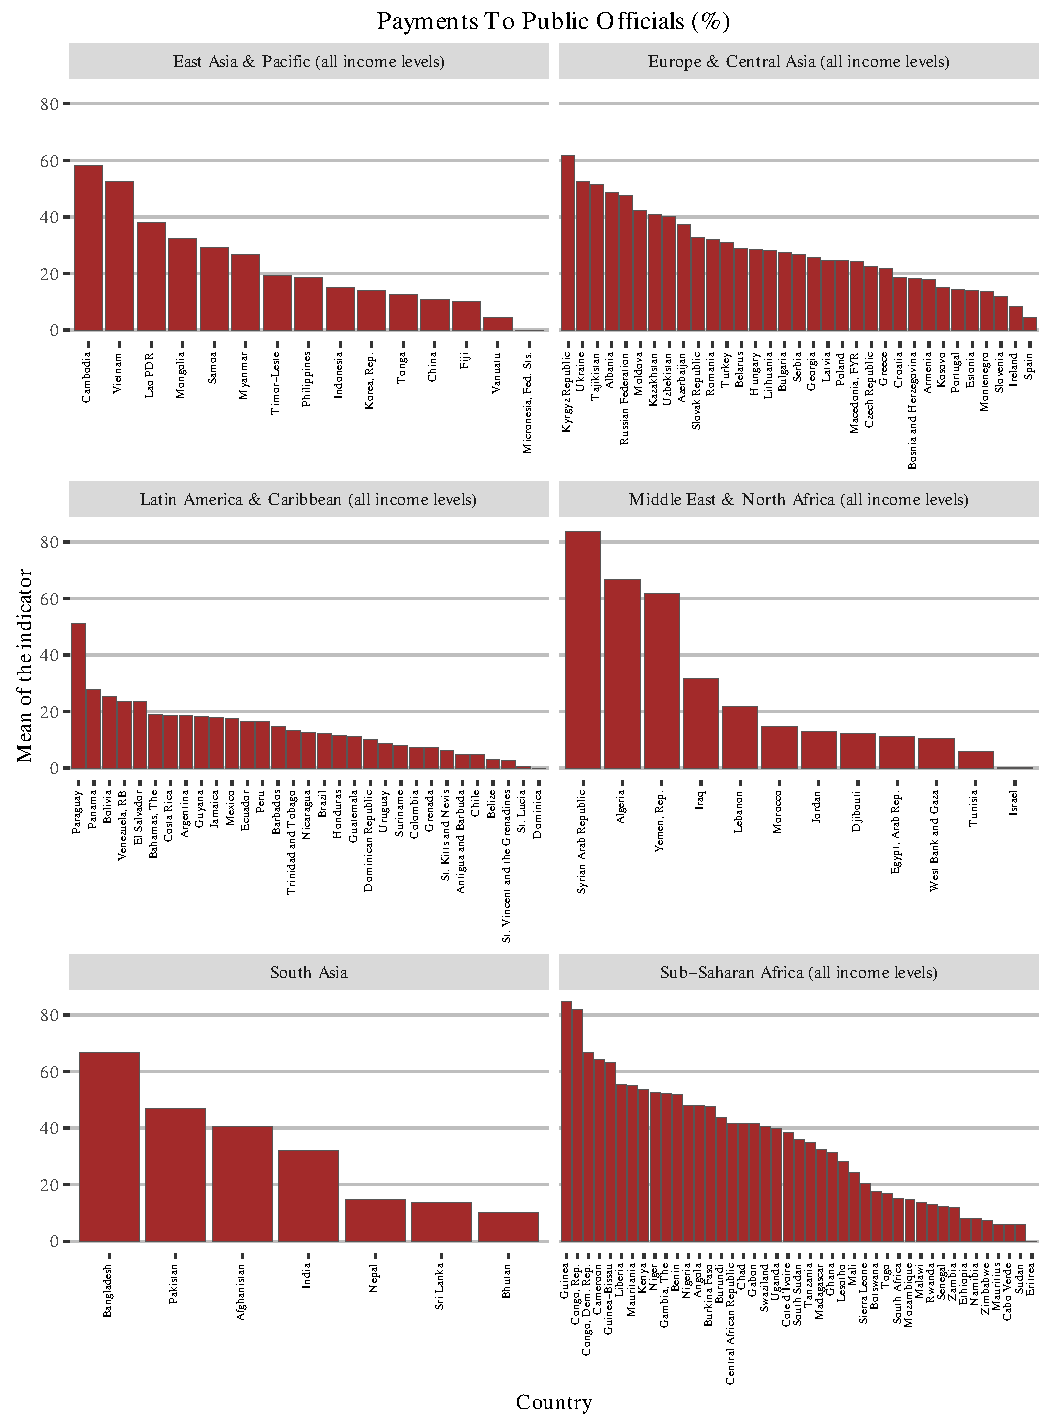
\includegraphics[max height=.9\textheight]{../img/wdi_payments_to_public_officials_perc.pdf}
\end{center}
\noindent \footnotesize{\textbf{Source:} Own creation and data obtained with package \texttt{WDI}, see the \cite{wb_r}.}
\end{figure}


\begin{figure}[H]
\begin{center}
\caption{WDI: Time to Enforce Contracts per Country/Region}
\label{fig_wdi_time_contract}
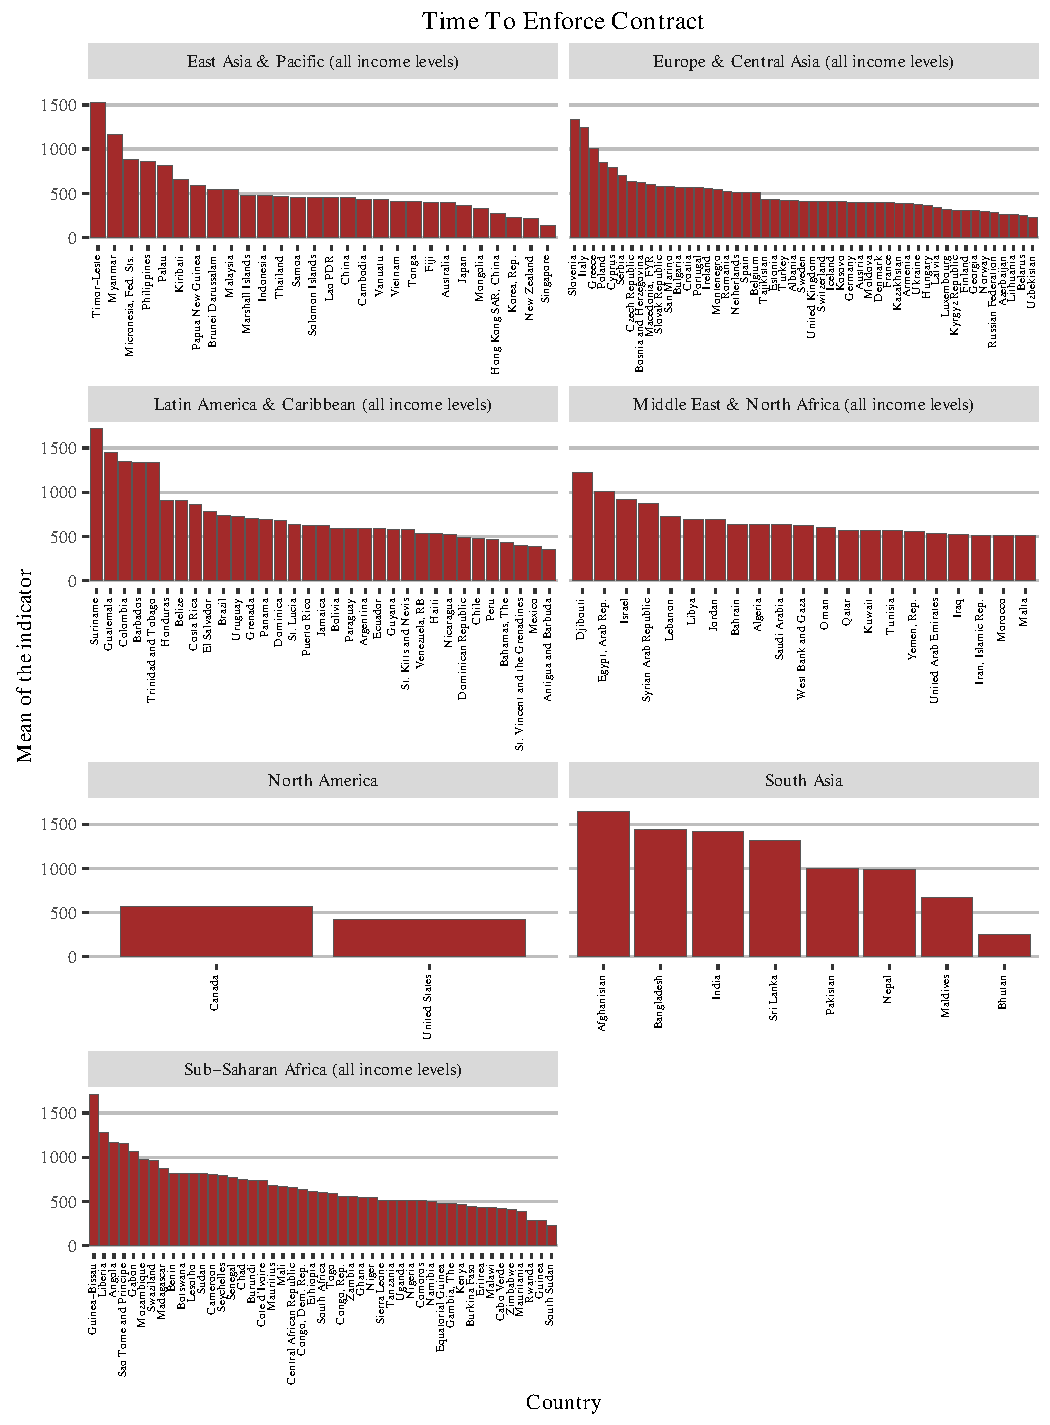
\includegraphics[max height=.9\textheight]{../img/wdi_time_to_enforce_contract.pdf}
\end{center}
\noindent \footnotesize{\textbf{Source:} Own creation and data obtained with package \texttt{WDI}, see the \cite{wb_r}.}
\end{figure}


\subsection{Major \& Historic Awards}

As it was explained previously, the other main public dataset was the Major and Historic contracts awards from the World Bank. The data include the variables shown in table \ref{tab_major_dict}. The variables shown refers to the names after an extensive cleaning process that involved merging data form all the Development Banks' sites and from the Historical Awards data obtained from the Wold Bank. Such variables include Procurement category that refers to whether if the procurement was  of  Consultant Services, Non-Consultant Services, Goods or Civil Works. The type of agreement refers to  International Bank for Reconstruction and Development (IBRD),  
Recipient-Executed Trust Funds (RETF), International Development Association (IDA), Institutional Development Fund (IDF), Global Environment Facility (GEF), State and Peace-Building Fund (SPF), California Air Resource Board (CARB) or Debt Reduction Facility (DRF) The Bid type can be Quality And Cost-Based Selection, Single Source Selection, Selection Based On Consultant's Qualification, Individual, National Competitive Bidding, International Competitive Bidding, CQS, SHOP, Direct Contracting, Quality Based Selection, Least Cost Selection, Selection Under a Fixed Budget, National Shopping, International Shopping or Limited International Bidding

The historical and mayor awards data has information of contracts awarded between 1986 to 2014. As it can be seen on figure \ref{fig_major_number} the historical awards correspond to years from 1986 to 1994 and the major awards are the ones from 1995 to June, 2014. Figure \ref{fig_major_number} shows that  the number of contracts have been reduced in the recent years in every region of the world and there was an abnormal amount of contracts awarded in the Latin America and Caribbean region between 1996 and 1999.  Figure \ref{fig_major_awarded_usd}  shows the total awarded amount of the Historical and Major contracts by each specific region. This figure shows that although the number of contracts was very high in the Latin America and Caribbean region in 1996 to 1999, the total awarded money to that region in US dollars was not as high as the number of contracts. 

% !TEX root = /Users/Carlos/Dropbox/detecting_collusion_corruption_fraud/latex_detecting_corruption_collusion_fraud/A0_thesis_detecting_collusion_corruption_fraud.tex
\begin{table}[H]
\begin{center}
\caption{Major and Historic Awards Dictionary} 
\label{tab_major_dict}
\scalebox{.7}{
\begin{tabular}{ll}
  \hline
Variable & Values \\ 
  \hline
agreement\_type & Agreement type \\ 
  award\_amount\_usd & Numeric \\ 
  award\_currency & USD \\ 
  award\_date & Date \\ 
  bider\_country\_2nd & Country \\ 
  bider\_country\_3rd & Country \\ 
  bider\_country\_4th & Country \\ 
  bid\_type & Type of Bid \\ 
  buyer & Name of the contractor \\ 
  buyer\_country & Country \\ 
  buyer\_country\_id & Country ID \\ 
  buyer\_reference & Identifier for the project \\ 
  competitive & Logical \\ 
  contract\_description & Description of the project \\ 
  domestic\_pref\_affect & Logical \\ 
  domestic\_pref\_allowed & Logical \\ 
  fiscal\_year & Date \\ 
  ln\_cr\_id & Loan ID \\ 
  major\_sector & Sector \\ 
  number\_of\_bids & Numeric \\ 
  number\_of\_firms & Numeric \\ 
  number\_of\_suppliers\_awarded & Numeric \\ 
  price\_escalating\_flag & Logical \\ 
  procurement\_category & Procurement Category \\ 
  product\_line\_original & Logical \\ 
  project\_id & Project ID \\ 
  project\_name & Project Name \\ 
  region & ECA, AFR, SAR, LCR, MNA, EAP, OTH \\ 
  sent\_date & Sent date \\ 
  signing\_date & Sign date \\ 
  supplier & Supplier name \\ 
  supplier\_country & Suplier Country \\ 
  supplier\_country\_id & Suplier Country ID \\ 
  unique\_id & Unique ID \\ 
  wb\_contract\_number & Contract Number \\ 
  historical & Logical \\ 
  country & Country \\ 
  year & Year \\ 
   \hline
   \footnotesize{\textbf{Source:} Own creation.} &

\end{tabular}}
\end{center}

\end{table}


\begin{figure}[H]
\begin{center}
\caption{Number of Historic \& Major awards per Region}
\label{fig_major_number}
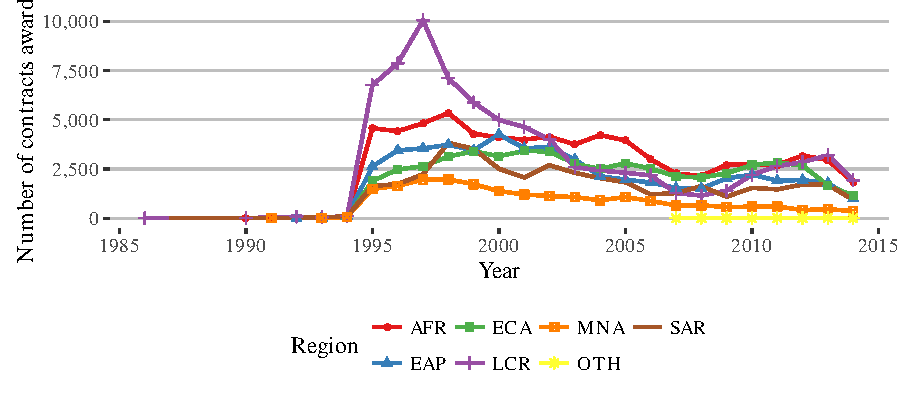
\includegraphics[max width=.95\textwidth]{../img/major_historic_region.pdf}
\end{center}
\noindent \footnotesize{\textbf{Source:} Own creation with data from the World Bank.}\\
\noindent \footnotesize{\textbf{Note:} OTH refers to projects that cannot be assigned to a specific country. Data to June, 2014.}
\end{figure}

\begin{figure}[H]
\begin{center}
\caption{Total awarded amount of Historic \& Major contracts per Region}
\label{fig_major_awarded_usd}
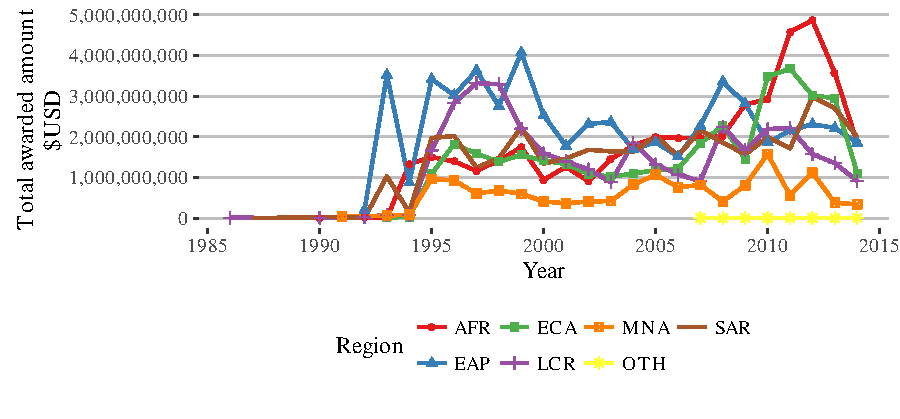
\includegraphics[max width=.95\textwidth]{../img/major_historic_region_awarded_usd.pdf}
\end{center}
\noindent \footnotesize{\textbf{Source:} Own creation with data from the World Bank.}\\
\noindent \footnotesize{\textbf{Note:} OTH refers to projects that cannot be assigned to a specific country. Data to June, 2014.}
\end{figure}


Figure \ref{fig_major_awarded_usd} also shows that just for 2013, the total awarded amount adds up to around 13,200 billion US dollars\footnote{1 billion = 1,000,000,000.} and that the awarded amount has increased more in Africa and in Europe from 2009 to 2013. 
It's important to notice that the data goes up to June, 2014 so the fall in the last point in figures  \ref{fig_major_number} and \ref{fig_major_awarded_usd} of each series for each region is not necessarily going down, it is probably better to ignore that data.

Now, figure \ref{fig_major_num_awarded_top} in  page \pageref{fig_major_num_awarded_top} shows the top six countries  in terms of awarded contracts. It is interesting how tendencies show the World Bank's priorities among time. For example, it is clear that the top countries from 2008 to 2015 has been Vietnam in first place, Afghanistan in second, and China and some Latin American countries in the next places. From 1998 to 2006, the tendencies were different, China and India take the first and second places with around 1,500 contracts per year for that period. In the next places, countries such as Brazil, Bosnia Herzegovina,  Argentina and the Russian Federation. Finally, in the term from 1990 to 1997, Mexico, Argentina and India take the first places followed by countries such as China, Bolivia, Ecuador, and other Latin American countries.

Next, figure \ref{fig_major_awarded_usd_top} in page \pageref{fig_major_awarded_usd_top} shows the top six countries  in terms of total awarded amount for each year in US dollars. From the figure, it is easy to see that China has been the country that has received the higher amount of money in contracts followed by India in second place and Brazil in third. This tend seems to be a constant in the top three countries since 1988 up to 2014. Other countries in the next three places include the Russian Federation, Vietnam, Africa and Africa.

The visualizations of  the data from figures such as \ref{fig_major_number} to  \ref{fig_major_awarded_usd_top} could help the World Bank to prioritize how to administer the number of contracts to award and the total awarded amount among different regions in the world and among different time period such that there's a balanced assignation of resources because figures  \ref{fig_major_number} to  \ref{fig_major_awarded_usd_top} suggest that the World Bank is not taking that into their assignation policy. This fact might or might not be related to how corruption, collusion and fraud but it certainly helps them as a political strategy.

\begin{figure}[H]
\begin{center}
\caption{Top six countries: number of awarded contracts}
\label{fig_major_num_awarded_top}
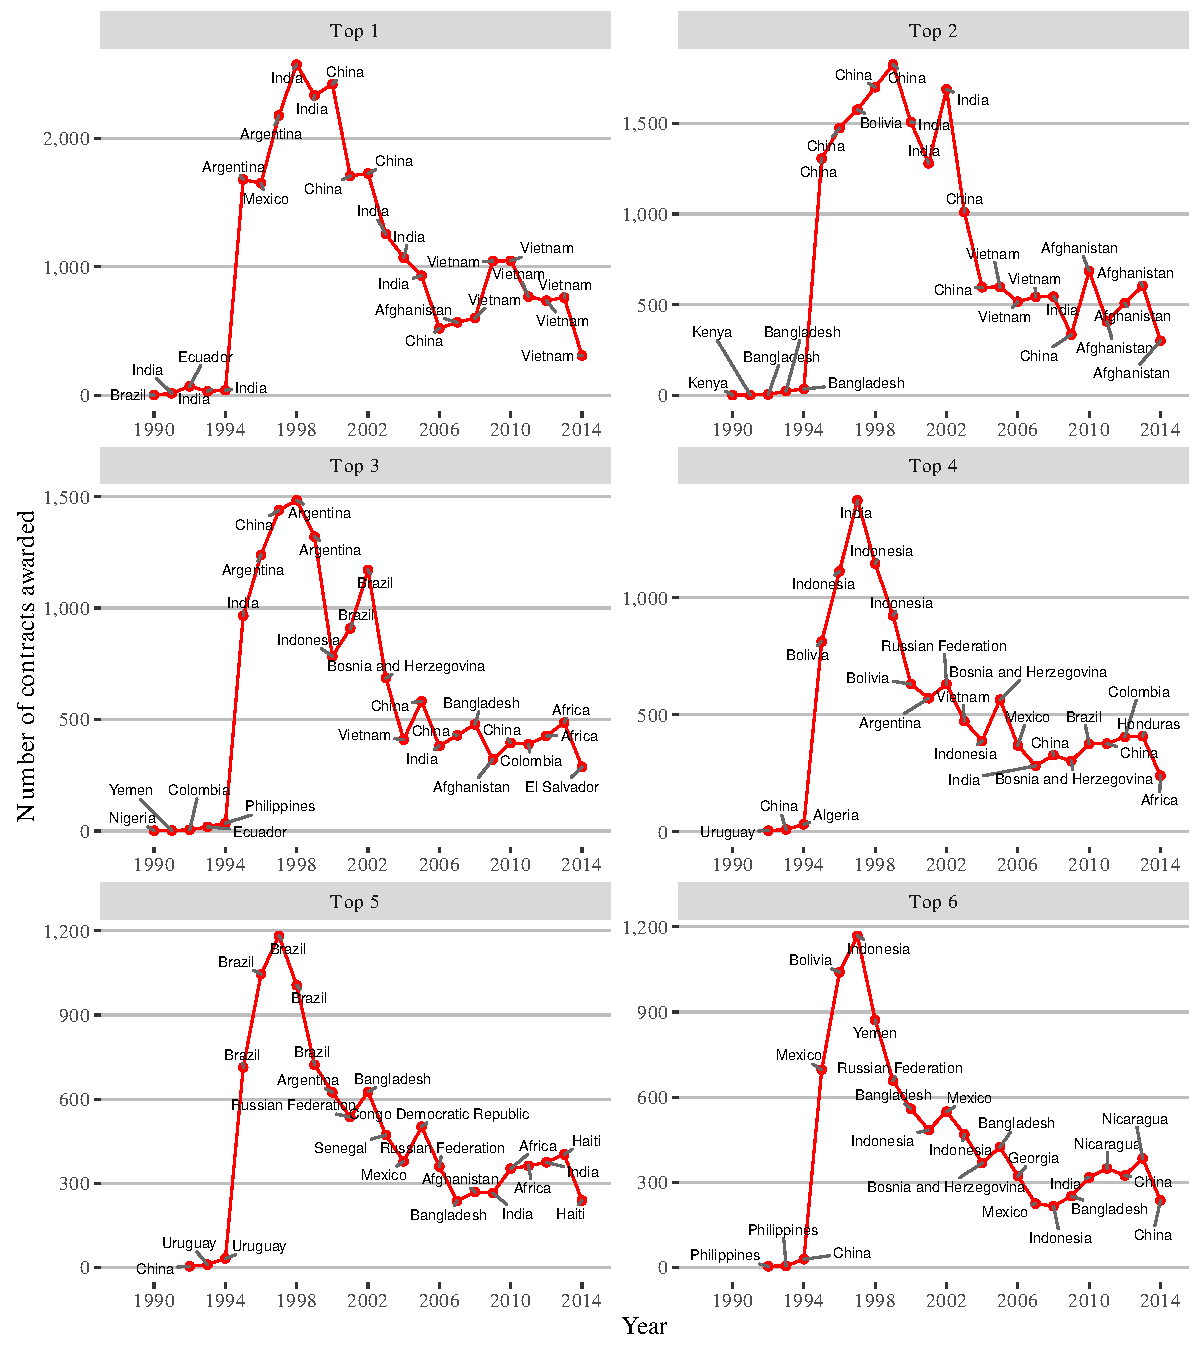
\includegraphics[max width=.95\textwidth]{../img/major_historic_top_contracts_awarded.pdf}
\end{center}
\noindent \footnotesize{\textbf{Source:} Own creation with data from the World Bank.}
\end{figure}



\begin{figure}[H]
\begin{center}
\caption{Top six countries: total awarded amount (\$USD)}
\label{fig_major_awarded_usd_top}
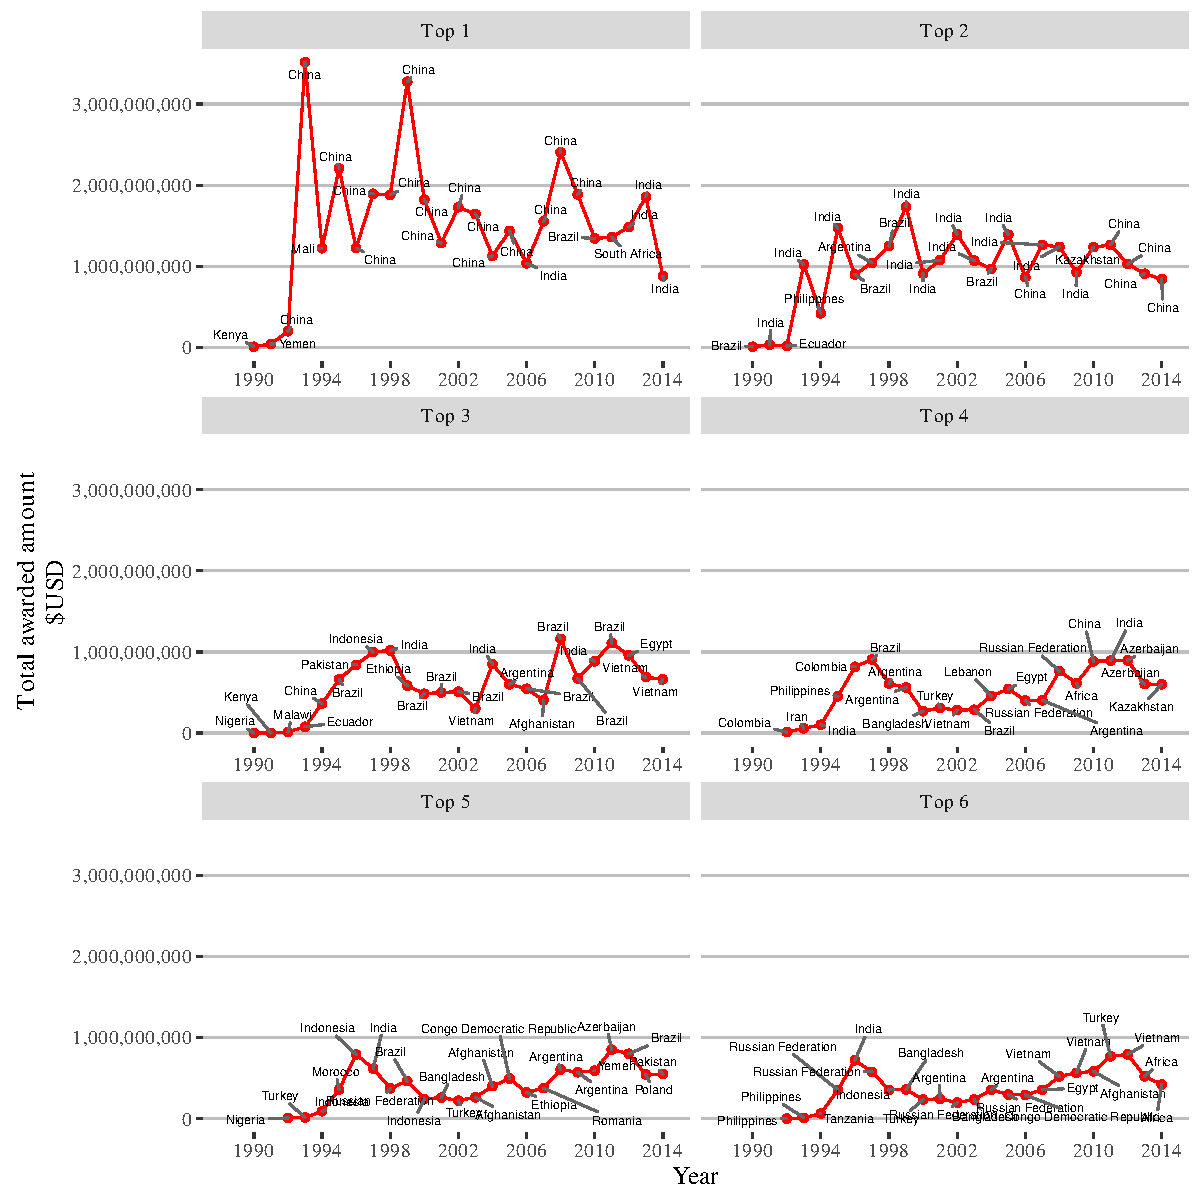
\includegraphics[max width=1\textwidth]{../img/major_historic_top_usd_awarded.pdf}
\end{center}
\noindent \footnotesize{\textbf{Source:} Own creation with data from the World Bank.}
\end{figure}

\newpage


\section{Entity names disambiguation}

As it was explained on chapter \ref{chap_procurements}, historically, the World Bank has made investigations based, mainly, on information and data provided third parties claiming that something is suspicions within a procurement process. Fortunately, the Wold Bank has been keeping record of the investigation process by generating the investigations data. The problem is that the information on the investigations data can not be easily linked to the Major and Historical awards since the suppliers, the bidders and the contractors' names were introduced in many different formats by many different organizations among the World Bank as described in chapter \ref{chap_intro}. This is a current limitation for the World Bank and a big problem regarding this project. This section explains one way to approach this problem.

The idea is very simple. Technology in modern search engines such as Google provides a reliable way to search for each one of the names registered in the data form the Investigations and the Major \& Historical awards data. So the plan was to \textit{google} each one of the unique names among the different data sources and compare the results so that entities that have similar results correspond to the same entity. This is a major data problem because it escalates very fast. After \textit{googleing} each one of the entities, results must be compared with all the remaining results in order to determine whether they are considered similar or not.  This means that if $n$ searches are made, then $n^2$ comparatives has to be computed. 

The first step then became very clear, removing words such that the problem could be simplified. This was referred as stop words removal. The idea behind removing the stop words is to simplify the work so that companies or entity names that are supposed to refer to the same organization or person but have different names among the data sources such as Price Waterhouse Coopers incorporated and Price Waterhouse Coopers INC actually do. By doing so, the entity names was reduced in about 15\% passing from 234,067 entity names originally to 198,957 unique values after removing punctuation and stop words, which is a very considerable amount taking into account that the idea is to search every one of them in Google.

The first problem then becomes that unique names from contractors, buyers and bidders ascend up to 198,957 unique names in the different data sources after cleaning for stop words and removing punctuation\footnote{The stop words were selected based on insight form the Integrity Vice Presidency. The stop words used were: \textit{`jsc', `corp', `m/s', `inc', `incorporated', `doo', `d.o.o.', `la', `el', `srl', `s.r.l.', `limited', `llc', `l.l.c.', `co', `corporation', `company', `ltd', `ltda', `lda', `de', `i/e', `ooo', `limited', `societe', `société', `et', `le', `and', `the', `of', `de', `des', `du', `sa', `s.a.', `pty', `ste', `sarl', `s.a.r.l.', `gmhb', `g.m.h.b.', `sprl', `s.p.r.l.'.} }. This has two main limitations, the first that, Google, does not allows users to perform computed searches that ascend to a number as big as what we are dealing here. The second, even if we were able to perform those searches, the number of binary comparatives to be made after the searches will be a number near to 39,204,000,000 which, if each binary computation lasted a 10\% of a second, it would take about 124 years to complete all of them sequentially, and,  of course, that is not useful at all.

Of course, the plan was not to perform sequential operations to make all the comparatives because, even if we had a 124 machines cluster to compute that in parallel, which is expensive enough, that process would still take about a year to end.

So the algorithm to approach this problem was the following: first, divide all the canonical names into several chunks and start an AWS machine, each with different I.P. address so that we don't face the restriction of making too much automated searches at Google; second, perform the searches for each one of the entity names and store the first 10 results given by google; third, after having the results within each chunk, compute the binary comparisons in that chunk to see how many searches in common entities have and if any two entities have the desired number of search results in common, group them as one company and then tag just one of them so that in the next step, fourth, the final step, just make the binary comparatives with the entities that had no matches and the ones tagged so that the process reduces the number of comparisons to be made. The code to perform this process is displayed in the  appendix \ref{chap_code} code \ref{code_seaches} and \ref{code_cluster_names}

Results were great because this algorithm completed in less than four days using about 450 instances. That means that a process that would normally take at least 100 days (by using 450 instances) was reduces in about 95\% the time making it very efficient. This was a great result because it created very useful results in a decent time for the project. Next subsection covers how to decide the parameters used for this process.

\subsection{Entity names disambiguation parameters \& results}

The results of the algorithm described in the last section and displayed in  the  appendix \ref{chap_code} code \ref{code_seaches} and \ref{code_cluster_names} depend on what is it considered to be a common entity name in terms of results in the Google searches. In other words, it depends on how many results of the Google searches in common are needed in order to consider two entities to be the same one.

Approaching this represent a trade-off between lowering the error in the number of unique entity names (false negatives) against being sure that two entities are actually the same in reality (false positives). For this project it was more relevant to reduce the false positives to be sure that whenever two entities have the same canonical name it's actually the case.

In order to decide how many searches in common were needed, we performed several experiments and talked with the partners at the Integrity Vice Presidency from the World Bank. They agreed that we needed a conservative approach to this problem. We tried using  nine, seven, five and three result searches in common within a random sample so that we could compare results in a viable time frame. Results using nine and seven searches in common seemed to bee too conservative. While, results using three results seemed desirable because it reduced the entity names in about 14\%, it seemed too relaxed for our partner at the World Bank so we decided to stay with five searches in common.  The total number of unique names was reduced in about 10\% which left us with great data for the next steps of the model.

The output of this algorithm was the first result of the project and this alone represented a first way to better understand procurement data among the different databases of the World Bank. Partners at the Integrity Vice Presidency were surprised that the project came up with a useful method to reconcile data that the investigators at the World Bank can actually use. The project itself could be just about a writing the best algorithm to reconcile entities among different databases that's why the investigators from the World Bank were thanked enough just for this results. It is very important to say that the output of this process is and will be used just as an additional tool that helps them  conduct their investigation process and in no way they are considering that the results of this process are absolute in any form.

Just to state a very clear example of how this algorithm worked, table	\ref{tab_disambiguation} shows all the suppliers that were matched to the entity Price Waterhouse Coopers.

% !TEX root = ../latex_detecting_corruption_collusion_fraud/A0_thesis_detecting_collusion_corruption_fraud.tex
\begin{filecontents}{longtab.tex}
\scriptsize
\begin{longtable}{XX}
\caption{Entity names disambiguation example} \\ 
  \hline
Supplier & Canonical Name \\ 
  \hline
\endhead
\hline
\multicolumn{2}{l}{\tiny Continues on next page}\endfoot
\multicolumn{2}{l}{\tiny End of table}\endlastfoot
 \hline
PRICE WATERHOUSE AUDITORES & PRICE WATER HOUSE COOPERS \\ 
  PRICE WATERHOUSE & PRICE WATER HOUSE COOPERS \\ 
  PRICE WATERHOUSE COOPERS & PRICE WATER HOUSE COOPERS \\ 
  PRICE WATERHOUSE/NORCONSULT & PRICE WATER HOUSE COOPERS \\ 
  PRICE WATERHOUSE COOPERS (PWC) & PRICE WATER HOUSE COOPERS \\ 
  PRICE WATERHOUSE COOPERS LIMITED & PRICE WATER HOUSE COOPERS \\ 
  PRICE WATERHOUSE COOPERS LTD. & PRICE WATER HOUSE COOPERS \\ 
  PRICE WATERHOUSECOOPERS PVT. LTD. & PRICE WATER HOUSE COOPERS \\ 
  MCO COOPERATING - PRICE WATER HOUSE & PRICE WATER HOUSE COOPERS \\ 
  PRICE WATERHOUSE COOPERS CONSULTANTS SINGAPORE PTE LTD & PRICE WATER HOUSE COOPERS \\ 
  SIR WILLIAM HALCROW/PRICE WATERHOUSE PAR & PRICE WATER HOUSE COOPERS \\ 
  PRICE WATERHOUSECOOPERS ASESORES GERENCIALES LTDA. & PRICE WATER HOUSE COOPERS \\ 
  PRICE WATERHOUSE COOPERS DEL ECUADOR & PRICE WATER HOUSE COOPERS \\ 
  PRICE WATERHOUSE S.C./TP/MA & PRICE WATER HOUSE COOPERS \\ 
  PRICE WATERHOUSE - AFRICA & PRICE WATER HOUSE COOPERS \\ 
  PRICE WATERHOUSE COOPERS ASSOCIATES AFRICA LTD. & PRICE WATER HOUSE COOPERS \\ 
  PRICE WATERHOUSE EASTERN EUROP & PRICE WATER HOUSE COOPERS \\ 
  PRICE WATERHOUSE/PR. WAT. \& CO & PRICE WATER HOUSE COOPERS \\ 
  A/O PRICE WATERHOUSE/PRICE WAT & PRICE WATER HOUSE COOPERS \\ 
  PRICE WATERHOUSE LLP, VA. USA & PRICE WATER HOUSE COOPERS \\ 
  PRICE WATERHOUSE - GMI AUDIT & PRICE WATER HOUSE COOPERS \\ 
  PRICE WATERHOUSE/COOPERS & PRICE WATER HOUSE COOPERS \\ 
  PRICE WATERHOUSE MEYERNEL & PRICE WATER HOUSE COOPERS \\ 
  PRICE WATERHOUSE PAN AFRICAN CONSULTANTS & PRICE WATER HOUSE COOPERS \\ 
  PRICE WATERHOUSE COOPERS AND HOWARD HUMPHREYS & PRICE WATER HOUSE COOPERS \\ 
  PISTRELLI, PRICE WHSE COOP\&LYB & PRICE WATER HOUSE COOPERS \\ 
  CENIT PRICE WATERHOUSE & PRICE WATER HOUSE COOPERS \\ 
  GMS SA - PRICE WATER & PRICE WATER HOUSE COOPERS \\ 
  PRICE WATERHOUSE \& CO. & PRICE WATER HOUSE COOPERS \\ 
  PRICE WATERHOUSE Y CO.,S.C. & PRICE WATER HOUSE COOPERS \\ 
  PRICE WATERHOUSE COOPERS CONSULTORES S.A. & PRICE WATER HOUSE COOPERS \\ 
  PRICE WATERHOUSE COOPERS Y COMPANIA, S.C. & PRICE WATER HOUSE COOPERS \\ 
  PRICE WATERHOUSE INTERAMERICAN & PRICE WATER HOUSE COOPERS \\ 
  PRICE WATERHOUSE COOPERS LLC & PRICE WATER HOUSE COOPERS \\ 
  CONSORTIUM ROTHSCHILD/LANDWELL \& ASSOCIES/PRICE WATERHOUSECO & PRICE WATER HOUSE COOPERS \\ 
  PW-PRICE WATERHOUSE & PRICE WATER HOUSE COOPERS \\ 
  PRICE WATER HOUSE COOPERS & PRICE WATER HOUSE COOPERS \\ 
  PRICE WATERHOUS COOPERS & PRICE WATER HOUSE COOPERS \\ 
  PLANT LOCATION INT'L/PRICE WA. & PRICE WATER HOUSE COOPERS \\ 
  BNP(PARIS)PRICE WATERHOUSE & PRICE WATER HOUSE COOPERS \\ 
  PRICE WATER HOUSE COOPERS LLP & PRICE WATER HOUSE COOPERS \\ 
  ROCHE/PRICE WATER HOUSE & PRICE WATER HOUSE COOPERS \\ 
  ROCHE INTER./PRICE WATERHOUSE & PRICE WATER HOUSE COOPERS \\ 
  PRICE WATERHOUSE COOPER LTD. & PRICE WATER HOUSE COOPERS \\ 
  PRICE WATERHOUSE COOPERS LAO LTD & PRICE WATER HOUSE COOPERS \\ 
  SAMIL PRICE WATERHOUSE COOPERS & PRICE WATER HOUSE COOPERS \\ 
  PRICE WATERHOUSECOOPERS & PRICE WATER HOUSE COOPERS \\ 
  PRICE WATERHOUSE COOPER VIETNAM & PRICE WATER HOUSE COOPERS \\ 
  PRICE WATERHOUSE LLC & PRICE WATER HOUSE COOPERS \\ 
  PRICE WATERHOUSE,SOFIA,BULGARI & PRICE WATER HOUSE COOPERS \\ 
  PRICE WATERHOUSE COOPERS KFT & PRICE WATER HOUSE COOPERS \\ 
  PRICE WATERHOUSE LLP & PRICE WATER HOUSE COOPERS \\ 
  PRICE WATERHOUSE COOPERS LLP & PRICE WATER HOUSE COOPERS \\ 
  PRICE WATERHOUSE COOPERS, UZBEK BRANCH & PRICE WATER HOUSE COOPERS \\ 
  PRICE WATER HOUSE & PRICE WATER HOUSE COOPERS \\ 
  PRICE WATERHOUSE S.A., & PRICE WATER HOUSE COOPERS \\ 
  PRICE WATERHOUSE/SABAS APPROTECH PROJECT & PRICE WATER HOUSE COOPERS \\ 
  PRICE WATERHOUSE/GONZ VILCHIS & PRICE WATER HOUSE COOPERS \\ 
  GONZALEZ VILCHIS/PRICE WATERHOUSE & PRICE WATER HOUSE COOPERS \\ 
  PRICE WATERHOUSE COOPERS N.V. & PRICE WATER HOUSE COOPERS \\ 
  PRICE WATERHOUSE COOPERS ANTIGUA & PRICE WATER HOUSE COOPERS \\ 
   \hline
\hline
\label{tab_disambiguation}
\end{longtable}

\end{filecontents}
\LTXtable{1.0\linewidth}{longtab.tex}

\section{Feature creation}















